\documentclass[tikz,border=5pt]{standalone}
\usepackage{amsmath}
\usetikzlibrary{arrows.meta,positioning,fit,backgrounds}

\definecolor{metayellow}{RGB}{255,250,181}
\definecolor{stagecyan}{RGB}{185,239,238}
\definecolor{queuegray}{RGB}{214,214,214}
\definecolor{countergreen}{RGB}{218,241,218}
\definecolor{softblue}{RGB}{225,239,250}

\begin{document}
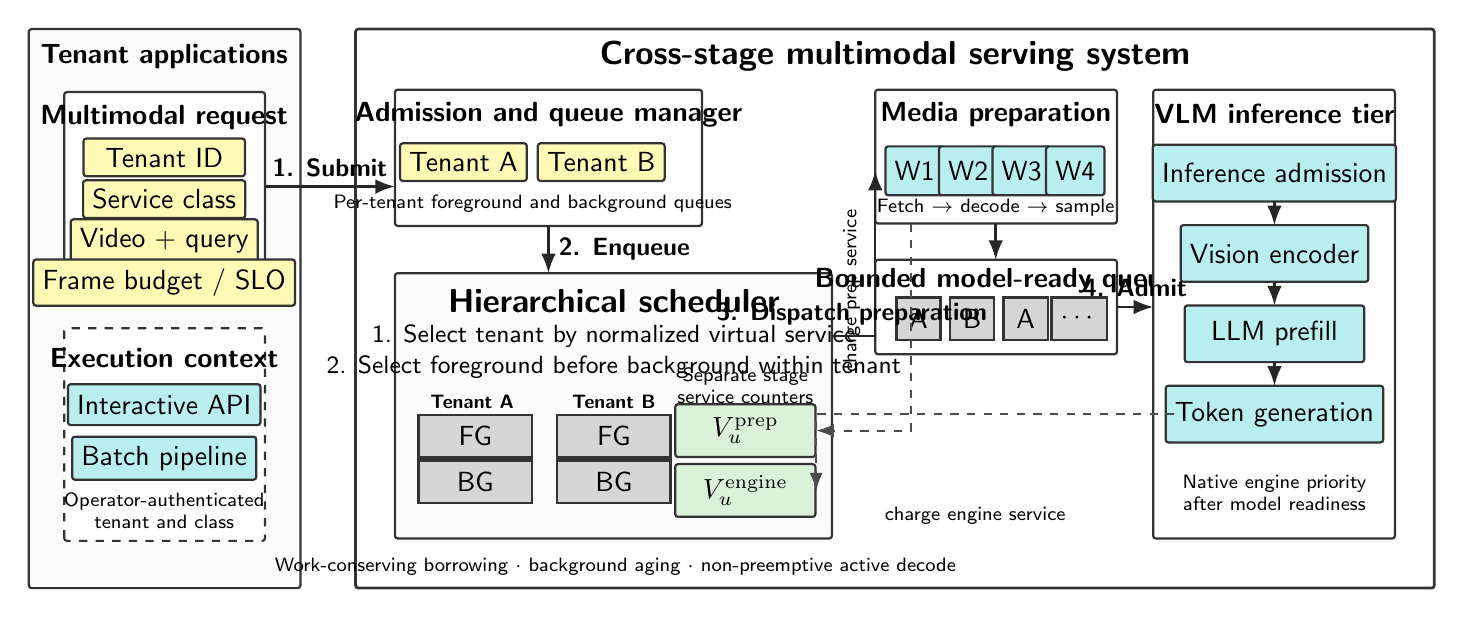
\begin{tikzpicture}[
  font=\sffamily,
  >=Latex,
  line/.style={draw=black!80, line width=0.8pt},
  arrow/.style={->, draw=black!85, line width=0.9pt},
  dashedarrow/.style={->, dashed, draw=black!70, line width=0.75pt},
  panel/.style={line, fill=white, rounded corners=1pt},
  stage/.style={line, fill=stagecyan, rounded corners=1pt, align=center},
  metadata/.style={line, fill=metayellow, rounded corners=1pt, align=center},
  qitem/.style={line, fill=queuegray, minimum height=0.54cm, align=center},
  counter/.style={line, fill=countergreen, rounded corners=1pt, align=center},
  label/.style={font=\bfseries\sffamily}
]

% Client side.
\draw[panel, fill=gray!3] (-0.1,-3.55) rectangle (3.35,3.55);
\node[label] at (1.62,3.20) {Tenant applications};

\draw[panel] (0.35,0.25) rectangle (2.90,2.75);
\node[label] at (1.62,2.43) {Multimodal request};
\node[metadata, minimum width=2.05cm, minimum height=0.43cm] at (1.62,1.92) {Tenant ID};
\node[metadata, minimum width=2.05cm, minimum height=0.43cm] at (1.62,1.39) {Service class};
\node[metadata, minimum width=2.05cm, minimum height=0.43cm] at (1.62,0.86) {Video + query};
\node[metadata, minimum width=2.05cm, minimum height=0.43cm] at (1.62,0.33) {Frame budget / SLO};

\draw[panel, dashed] (0.35,-2.95) rectangle (2.90,-0.25);
\node[label] at (1.62,-0.62) {Execution context};
\node[stage, minimum width=2.05cm, minimum height=0.52cm] at (1.62,-1.22) {Interactive API};
\node[stage, minimum width=2.05cm, minimum height=0.52cm] at (1.62,-1.90) {Batch pipeline};
\node[align=center, font=\scriptsize\sffamily] at (1.62,-2.57)
  {Operator-authenticated\\tenant and class};

% Server boundary.
\draw[panel, line width=1pt] (4.05,-3.55) rectangle (17.75,3.55);
\node[label, font=\large\bfseries\sffamily] at (10.90,3.20)
  {Cross-stage multimodal serving system};

% Admission and queue manager.
\draw[panel] (4.55,1.05) rectangle (8.45,2.78);
\node[label] at (6.50,2.47) {Admission and queue manager};
\node[metadata, minimum width=1.45cm, minimum height=0.43cm] at (5.42,1.86) {Tenant A};
\node[metadata, minimum width=1.45cm, minimum height=0.43cm] at (7.17,1.86) {Tenant B};
\node[font=\scriptsize\sffamily] at (6.30,1.33)
  {Per-tenant foreground and background queues};

% Hierarchical scheduler.
\draw[panel, fill=gray!2] (4.55,-2.92) rectangle (10.10,0.45);
\node[label, font=\large\bfseries\sffamily] at (7.33,0.10)
  {Hierarchical scheduler};
\node[font=\small\sffamily] at (7.33,-0.35)
  {1. Select tenant by normalized virtual service};
\node[font=\small\sffamily] at (7.33,-0.74)
  {2. Select foreground before background within tenant};

\node[font=\scriptsize\bfseries\sffamily] at (5.53,-1.18) {Tenant A};
\node[qitem, minimum width=1.44cm] at (5.57,-1.62) {FG};
\node[qitem, minimum width=1.44cm] at (5.57,-2.20) {BG};
\node[font=\scriptsize\bfseries\sffamily] at (7.33,-1.18) {Tenant B};
\node[qitem, minimum width=1.44cm] at (7.33,-1.62) {FG};
\node[qitem, minimum width=1.44cm] at (7.33,-2.20) {BG};

\node[counter, minimum width=1.78cm, minimum height=0.67cm] at (9.00,-1.55)
  {$V_u^{\mathrm{prep}}$};
\node[counter, minimum width=1.78cm, minimum height=0.67cm] at (9.00,-2.31)
  {$V_u^{\mathrm{engine}}$};
\node[font=\scriptsize\sffamily, align=center] at (9.00,-0.98)
  {Separate stage\\service counters};

% Preparation tier.
\draw[panel] (10.65,1.08) rectangle (13.72,2.78);
\node[label] at (12.18,2.47) {Media preparation};
\node[stage, minimum width=0.56cm, minimum height=0.62cm] at (11.15,1.75) {W1};
\node[stage, minimum width=0.56cm, minimum height=0.62cm] at (11.83,1.75) {W2};
\node[stage, minimum width=0.56cm, minimum height=0.62cm] at (12.51,1.75) {W3};
\node[stage, minimum width=0.56cm, minimum height=0.62cm] at (13.19,1.75) {W4};
\node[font=\scriptsize\sffamily] at (12.18,1.28)
  {Fetch $\rightarrow$ decode $\rightarrow$ sample};

% Model-ready queue.
\draw[panel] (10.65,-0.58) rectangle (13.72,0.62);
\node[label] at (12.18,0.35) {Bounded model-ready queue};
\node[qitem, minimum width=0.56cm] at (11.20,-0.13) {A};
\node[qitem, minimum width=0.56cm] at (11.88,-0.13) {B};
\node[qitem, minimum width=0.56cm] at (12.56,-0.13) {A};
\node[qitem, minimum width=0.56cm] at (13.24,-0.13) {$\cdots$};

% Inference tier.
\draw[panel] (14.18,-2.92) rectangle (17.25,2.78);
\node[label] at (15.72,2.47) {VLM inference tier};
\node[stage, minimum width=2.28cm, minimum height=0.72cm] at (15.72,1.72)
  {Inference admission};
\node[stage, minimum width=2.28cm, minimum height=0.72cm] at (15.72,0.70)
  {Vision encoder};
\node[stage, minimum width=2.28cm, minimum height=0.72cm] at (15.72,-0.32)
  {LLM prefill};
\node[stage, minimum width=2.28cm, minimum height=0.72cm] at (15.72,-1.34)
  {Token generation};
\node[font=\scriptsize\sffamily, align=center] at (15.72,-2.34)
  {Native engine priority\\after model readiness};

% Main numbered flow.
\draw[arrow] (2.90,1.55) -- node[above, font=\bfseries\small\sffamily]
  {1. Submit} (4.55,1.55);
\draw[arrow] (6.50,1.05) -- node[right, font=\bfseries\small\sffamily]
  {2. Enqueue} (6.50,0.45);
\draw[arrow] (10.10,-0.35) -| node[pos=0.23, above, font=\bfseries\small\sffamily]
  {3. Dispatch preparation} (10.65,1.75);
\draw[arrow] (12.18,1.08) -- (12.18,0.62);
\draw[arrow] (13.72,0.02) -- node[above, font=\bfseries\small\sffamily]
  {4. Admit} (14.18,0.02);
\draw[arrow] (15.72,1.36) -- (15.72,1.06);
\draw[arrow] (15.72,0.34) -- (15.72,0.04);
\draw[arrow] (15.72,-0.68) -- (15.72,-0.98);

% Accounting feedback.
\draw[dashedarrow] (11.10,1.08) |- (9.90,-1.55);
\draw[dashedarrow] (14.45,-1.34) -| (9.90,-2.31);
\node[font=\scriptsize\sffamily, rotate=90] at (10.35,0.22) {charge prep service};
\node[font=\scriptsize\sffamily] at (11.92,-2.63) {charge engine service};

% Policy properties.
\node[align=center, font=\scriptsize\sffamily] at (7.35,-3.28)
  {Work-conserving borrowing $\cdot$ background aging $\cdot$ non-preemptive active decode};

\end{tikzpicture}
\end{document}
